\section{Lighting}
\subsection{Modelli Matematici della luce}
\begin{enumerate}
    \item \textbf{Ottica geometrica}: la luce è modellata utilizzando raggi. I raggi seguono regole geometriche. L'ottica geometrica può modellare diversi effetti luminosi come la riflessione e la rifrazione.
    
    \item \textbf{Ottica ondulatoria}: la luce è modellata come un'onda che si propaga. L'ottica ondulatoria può modellare effetti luminosi come la diffrazione.
    
    \item \textbf{Ottica elettromagnetica}: può descrivere effetti luminosi come la polarizzazione della luce, non spiegata dall'ottica ondulatoria.
    
    \item \textbf{Ottica dei fotoni}: la meccanica quantistica viene utilizzata per modellare gli effetti luminosi.
\end{enumerate}
La luce energetica è emessa da una sorgente di luce, questa viaggia attraverso la scena e interagisce con la scena finchè non si stabilizza.
Questo prceeso accade alla velocità della luce. Quindi, per noi, tutto questo processo è stabile\\ Cosa succede quando un raggio di luce colpisce una superficie?
\begin{figure}[H]
    \centering
    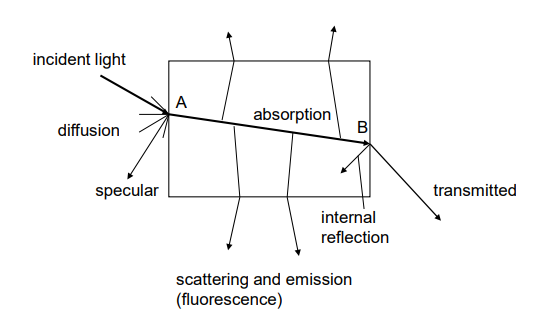
\includegraphics[width=0.5\textwidth]{images/LightMat.png} 
    \caption{Light-material interaction}
    \label{fig:immagine}
\end{figure}

\subsection{Solid angle}
Rappresenta la dimensione angolare di un conoide infinitesimale lungo una data direzione.
Può essere interpretato come una direzione associata a un'area infinitesimale sulla sfera unitaria (unità di misura: steradianti).
È l'estensione nello spazio tridimensionale del concetto di angolo planare.
$\theta$ è misurato in radianti come il rapporto $\frac{s}{r}$, dove $s$ è la lunghezza dell'arco di un cerchio di raggio $r$ sotteso da $\theta$.
Analogamente, $\Omega$ è misurato in steradianti come il rapporto $\frac{A}{r^2}$, dove $A$ è l'area superficiale di una sfera di raggio $r$ sottesa da $\Omega$.

Esempi:
\begin{itemize}
    \item Angolo retto: $\frac{2 \pi r}{4 r} = \frac{\pi}{2}$ radianti
    \item Angolo solido di un'emisfero: $\frac{4 \pi r^2}{2 r^2} = 2 \pi$ steradianti
\end{itemize}
\subsection{Radiometry}
\textbf{Flusso radiante} (watt) è l'energia radiante che attraversa una superficie nell'unità di tempo:
$\Phi= \frac{dQ}{dt} $ \\
\textbf{Irradianza (E)} (watt/m2) è il flusso radiante incidente su un elemento di superficie:
$E(x)= \frac{d\Phi}{dA} $ \\
\textbf{La radianza (L)} (watt/m2sr) è il flusso radiante per angolo solido per unità di area
$L(x,\vec{w})= \frac{d^2\phi}{\cos\theta dwdA} $ \\
L'irradianza (E(x)) è data dall'integrale della radianza incidente (L) lungo tutte le direzioni.
Il flusso radiante è dato dall'integrale della radianza incidente (L) lungo tutte le direzioni e dall'area considerata.
$E(x)=\int_{\Omega}{} L(x,\vec{w'})(\vec{w'}\cdot n)d\vec{w'} \, $ \\
Una sorgente luminosa puntiforme emette uniformemente la luce in tutte le direzioni, producendo: \\
$E(x)=\frac{\Phi_s \cos \theta}{4\pi r^2 }$ \\
\textbf{L'intensità della luce diminuisce con il quadrato della distanza.}
\subsection{e BSSRDF (Bidirectional Scattering Surface Reflectance Distribution Function)}
Quando la luce colpisce una superficie interagisce con essa e, nel caso generale, esce dalla superficie da una posizione diversa da quella di ingresso (dispersione).
Il \textbf{BSSRDF} (Bidirectional Scattering Surface Reflectance Distribution Function) è una funzione che descrive il processo di dispersione.
Il BSSRDF può essere scritto come: \\
$S(x_i,\vec{w_i},x_r,\vec{w_r})=\frac{dL_r(x_r,\vec{w_r})}{d\Phi_i(x_i,\vec{w_i})}$ \\
Dove $L_r$ rappresenta la radianza uscente dal punto $x_r$ nella direzione $w_r$ e $\Phi_i$ è il flusso radiante incidente nel punto $x_i$ dalla direzione $w_i$.
È una funzione di otto parametri! (due parametri per identificare una posizione sulla superficie e due angoli per specificare una direzione nelle coordinate sferiche).
\\
La BRDF (Bidirectional Reflectance Distribution Function) è un'approssimazione del BSSRDF per descrivere la riflessione della luce da parte di una superficie.
In particolare, la BRDF è il rapporto tra la radianza uscente (luce riflessa) in una certa direzione e in un dato punto della superficie (x) e l'irradianza incidente nello stesso punto proveniente da una direzione specifica.
\\
$f_r(x,\vec{w_i},\vec{w_r})=\frac{dL_r(x,\vec{w_r})}{dE_i(x,\vec{w_i})}=\frac{dL_r(x,\vec{w_r})}{L_i(x,\vec{w_i})(\vec{w_i}\cdot\vec{n} )d\vec{w_i}}$
\subsection{The Rendering Equation}
\begin{figure}[H]
    \centering
    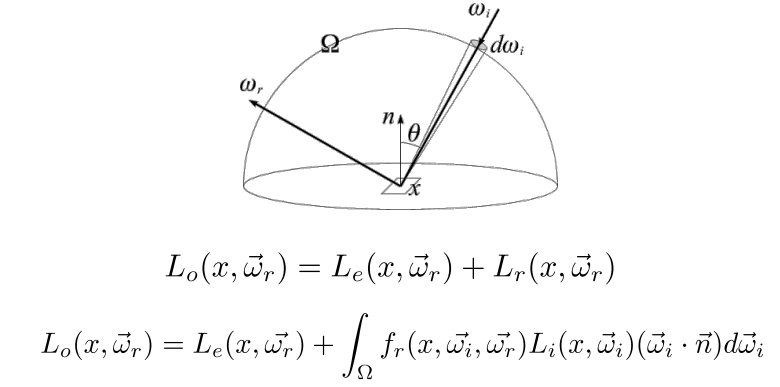
\includegraphics[width=0.5\textwidth]{images/RendEq.png} 
    \caption{Rendering Equations}
    \label{fig:immagine}
\end{figure}
La luce visibile in un punto della scena per una direzione specifica è data dalla luce emessa più la luce riflessa in quella direzione.
\\
$L_o(x,\vec{w_r})=L_e(x,\vec{w_r})+L_r(x,\vec{w_r})$
\\
La luce riflessa è ottenuta integrando tutte le contribuzioni ponderate in base alla BRDF (che dipende dal materiale specifico) e agli angoli di riflessione
$L_o(x,\vec{w_r})=L_e(x,\vec{w_r})+ \int_{\Omega}{}f_r(x,\vec{w_i},\vec{w_r})L_i(x,\vec{w_i})(\vec{w_i},\vec{n})d\vec{w_i}$ \\
$x$ \ Punto sulla superficie dove viene calcolata l'equazione\\
$\vec{w_r}$ \ Direzione della radianza riflessa;\\
$\vec{w_i}$  \ Direzione del raggio luminoso incidente (radianza in ingresso)\\
$f_r$ \ \vspace{10pt} Funzione che determina la frazione della luce riflessa\\
$\vec{w_i}\cdot\vec{n}$  \ \vspace{10pt} Coseno dell'angolo di incidenza (rispetto alla normale della superficie)\\
La computazione dell'Equazione di Rendering è molto dispendiosa
È necessario calcolarla diverse volte per molte parti della scena
La soluzione è utilizzare un modello di illuminazione locale
Semplificazione (approssimazione)
Vengono modellati solo gli effetti locali
\subsubsection{Local and Global effects}
Gli effetti visivi causati dalla luce possono essere suddivisi in effetti locali o globali.
\begin{itemize}
    \item \textbf{Modello di illuminazione}: formulazione matematica dell'equazione dell'illuminazione. Tipicamente, i modelli di illuminazione sono approssimazioni dell'Equazione di Rendering.
    \item \textbf{Illuminazione}: calcolo della luce.
    \item \textbf{Shading}: calcolo del colore di ciascun pixel.
\end{itemize}
\subsubsection{Phong Lighting model}
Creato da Phong Bui-Tuong attorno al 1975, semplifica l'interazione 
Simula l'interazione luce-materiale con materiali opachi.
\begin{itemize}
    \item La rifrazione non è modellata: non può essere utilizzata per materiali semitrasparenti o trasparenti.
    \item Piuttosto realistico... Ma alcuni materiali sembrano plastica.
    \item È composto da tre termini: un termine che modella la componente diffusa del materiale, un termine che modella la componente speculare del materiale e un termine ambientale che cattura le inter-riflessioni della scena.
\end{itemize}
L'obbiettivo è approssimare il \textbf{brdf}, il metodo è quello di semplificare la legge fisica che sta dietro alla specular reflection e la diffuse reflection.
\subsubsection{Fresnel Law}
Quando un raggio di luce passa da un mezzo all'altro con diverso indice di rifrazione, alla superficie di separazione una parte del raggio viene riflesso e una parte viene trasmesso. La somma dell'energia dei due raggi è uguale all'energia del raggio originale.
Se non c'è rifrazione dall'aria all'oggetto solido, il raggio viene interamente riflesso. L'angolo di riflessione è uguale all'angolo di incidenza. Questo principio è valido per materiali lisci e lucidi.
\subsubsection{Lambert Law}
I materiali opachi (es. legno, pietra) sono caratterizzati da una superficie con faccette microscopiche che riflettono la luce in modo casuale in ogni direzione. A livello macroscopico, la luce viene riflessa uniformemente in tutte le direzioni, con un'intensità proporzionale alla direzione del raggio incidente e alla normale della superficie.
\subsubsection{Diffuse Reflection}
Sorgenti luminose puntiformi sono caratterizzate da:
\begin{itemize}
    \item La posizione $P$
    \item L'intensità della luce emessa $I_P$
\end{itemize}

La direzione della luce incidente è: \\
$ \vec{L}=|L-P| $ \\ 
Tenendo conto dell'angolo Illuminazione: \\
$ \cos(\theta)= \vec{L}\cdot \vec{N}  $ \\
La funzione di riflessione è approssimata come una costante $k_d$ che dipende dal materiale.\\
Equazione dell'illuminazione (diffusa):
$I=I_p k_d \cos \theta$ \\
or \\
$I=I_p k_d \vec{N}\cdot\vec{L}$
Dobbiamo ottenere il massimo tra il coseno e zero nella formula precedente. \\
$I=I_p k_d max(0,\cos \theta)=I_p k_d \cos(0,\vec{N} \cdot \vec{L}) $ \\
\subsubsection{Specular Reflection}
Riflettore non ideale:
Un'approssimazione più realistica rispetto alla legge di Fresnel
-> evidenza speculare
In pratica, l'evidenza speculare è data dalla luce riflessa nella direzione dell'osservatore, il che significa che la sua posizione sull'oggetto dipende dall'osservatore.
L'aspetto di un oggetto opaco (riflessione diffusa solamente) non dipende dalla posizione dell'osservatore.
C'è una dipendenza dall'angolo tra la direzione di riflessione ideale R e la direzione della vista V.
Massima riflessione per a = 0
Rapido decadimento quando i valori di alfa aumentano.
Questo decadimento è modellato con un esponente (n) applicato al coseno dell'angolo $\alpha$.
Il parametro n è l'esponente della riflessione speculare del materiale.
Il vettore R è calcolato come: \\
$\vec{R}=2v \vec{N} ( \vec{N} \cdot \vec{L})- \vec{L}$ \\
L'equazione dell'illuminazione per la riflessione speculare solamente: \\
$I=I_pk_s cos^n\alpha $ \\
Il parametro $k_s$ caratterizza il materiale speculare, insieme all'esponente n.
\subsubsection{Ambient Component}
Le inter-riflessioni tra gli oggetti diversi della scena non sono modellate dal modello di Phong.
Le inter-riflessioni possono essere approssimate dal seguente componente: \\
$I=I_a k_a $\\
\begin{itemize}
    \item $I$ rappresenta il totale dell'energia radiante emessa dalla scena
    \item $K_a$ modella la riflettività del materiale
    \item $I_a$ è costante per tutti i punti della scena.
\end{itemize}
La luce ambientale aggiunge realismo alla scena, anche se è un'approssimazione approssimativa dell'illuminazione indiretta
Tutte le contribuzioni descritte vengono sommate insieme per formare l'equazione dell'illuminazione.
Dobbiamo sommare la luce per ciascuna sorgente luminosa presente nella scena.
\begin{figure}[H]
    \centering
    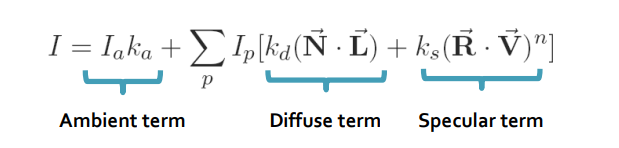
\includegraphics[width=0.5\textwidth]{images/Summation.png} 
    \caption{Summation}
    \label{fig:immagine}
\end{figure}
È possibile tenere conto dell'attenuazione della luce dovuta alla distanza. \\
\\
$I=I_ak_a+ \sum_{p}{} f_{att_p} I_p[k_d(\vec{N}\cdot\vec{L})+k_s(\vec{R}\cdot\vec{V})^n] $
\\
Considerando una rappresentazione RGB, l'equazione deve essere elaborata separatamente per ogni componente cromatica.\\

$I_r=I_{a,r}k_{a,r}+I_{p,r}[k_{d,r}(\vec{N}\cdot\vec{L})+k_{s,r}(\vec{R}\cdot\vec{V})^n]$\\
$I_g=I_{a,g}k_{a,g}+I_{p,g}[k_{d,g}(\vec{N}\cdot\vec{L})+k_{s,g}(\vec{R}\cdot\vec{V})^n]$\\
$I_b=I_{a,b}k_{a,b}+I_{p,b}[k_{d,b}(\vec{N}\cdot\vec{L})+k_{s,b}(\vec{R}\cdot\vec{V})^n]$\\
\subsubsection{Shading}
Il modello di illuminazione di Phong ci spiega come calcolare l'interazione tra la luce e il materiale senza utilizzare l'Equazione di Rendering (troppo complessa).
Ora, vedremo dove calcolare l'equazione (per ogni faccia? per ogni vertice?).
Problema del \textbf{Flat Shading} :La discretizzazione non rappresenta bene la continuità sulla superficie.
\begin{figure}[H]
    \centering
    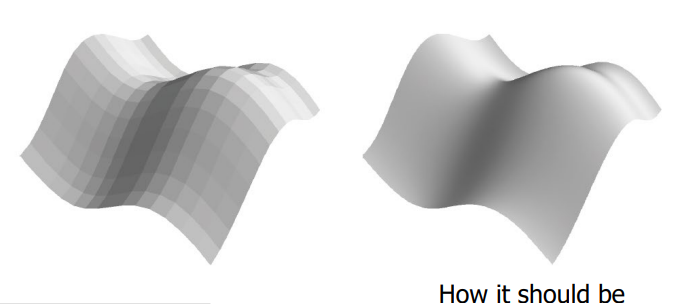
\includegraphics[width=0.5\textwidth]{images/Shading.png} 
    \caption{Flat Shading}
    \label{fig:immagine}
\end{figure}
Soluzione: Userò un'enorme quantità di facce...
NON FUNZIONA! Le discontinuità tra le facce sono sempre visibili a causa dell'effetto visivo della Mach Banding. \\
\begin{figure}[H]
    \centering
    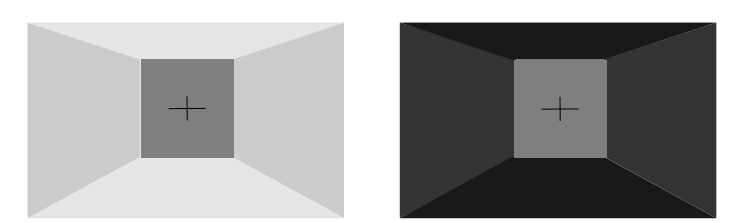
\includegraphics[width=0.5\textwidth]{images/MatchBand.png} 
    \caption{Mach Banding}
    \label{fig:immagine}
\end{figure}
\section{Gouraud Shading}

I contrasti locali cambiano la nostra percezione.
Un oggetto vicino a un oggetto luminoso appare più scuro, un oggetto vicino a un oggetto scuro appare più chiaro.
Calcolare l'illuminazione solo in alcuni punti Interpolazione lineare
L'interpolazione può essere calcolata durante la rasterizzazione in modo semplice ed efficiente.
Lo shading può essere aggiornato incrementalmente durante la rasterizzazione.\\
\textbf{Vertex Normal}:
\begin{itemize}
    \item La normale della faccia è ben definita.
    \item Un modo è calcolare la normale del vertice come la media delle normali delle facce incidenti sul vertice.
\end{itemize}
$\vec{N_v}=\frac{ \sum_{i}{}\vec{N_i} }{| \sum{_i}{}\vec{N_i} |}$ \\
\begin{figure}[H]
    \centering
    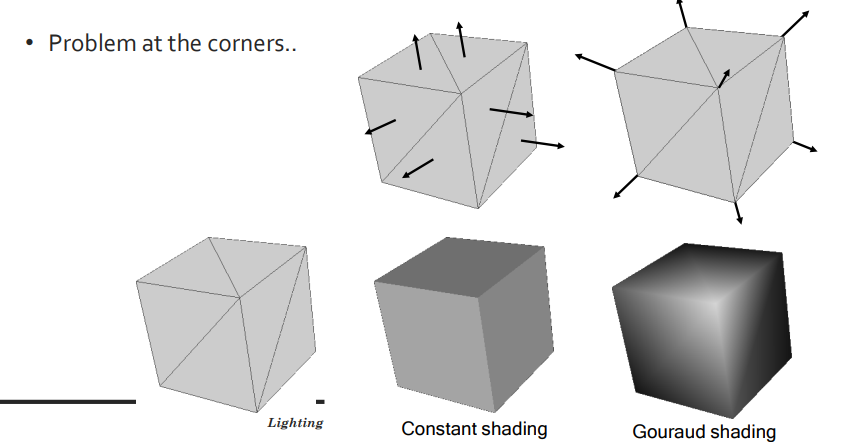
\includegraphics[width=0.5\textwidth]{images/AngleProblems.png} 
    \caption{Limitazione }
    \label{fig:immagine}
\end{figure}
Si può utilizzare il Gouraud Shading, Soluzione: utilizzare normali diverse per le diverse facce degli angoli.
La struttura dati dovrebbe tenerne conto.
\begin{figure}[H]
    \centering
    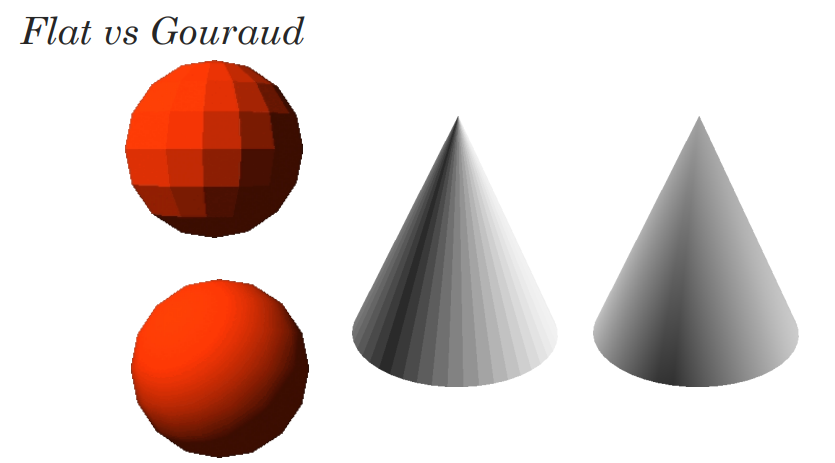
\includegraphics[width=0.5\textwidth]{images/FlatvsGround.png} 
    \caption{Flat vs Gouraud }
    \label{fig:immagine}
\end{figure}
\subsubsection{Phong Shading}
Shading di Gouraud: ottimo rapporto tra complessità e qualità del risultato finale.
\begin{itemize}
    \item Il risultato finale non è buono per superfici con un alto coefficiente speculare.
    \item Problema: con un alto indice di riflessione ($n$), le dimensioni dell'illuminazione speculare sono ridotte; utilizzando questa tecnica di shading, l'illuminazione speculare potrebbe propagarsi sull'intera faccia (a causa dell'interpolazione). L'illuminazione speculare non viene disegnata se è all'interno di una faccia.
\end{itemize}
\textbf{Soluzione}: le normali delle superfici vengono interpolate e l'equazione di illuminazione viene calcolata per ogni pixel.